\documentclass{exos}
\usepackage{main}

\begin{document}
\begin{exercize}
Soit $f : x \mapsto 2x - 230 + \dfrac{7200}{x}$.
\begin{alphaquestions}
\item On admet que $f$ est dérivable sur $[30;120]$. Montrer que pour tout $x$ dans $[30;120]$,
\begin{equation*}
f'(x)=2 - \dfrac{7200}{x^2}
\end{equation*}
\item En déduire que pour tout $x$ dans $[30;120]$,
\begin{equation*}
f'(x) = \dfrac{2(x-60)(x + 60)}{x^2}
\end{equation*}
\item Compléter le tableau de signes de $f'$ et le tableau de variations de $f$ :
\begin{center}
\begin{tikzpicture}
\tkzTabInit{$x$/1, Signe de $x-60$/1, Signe de $x + 60$/1, Signe de $f'$/2, Variations de $f$/2}{$30$,\dots,\dots,$120$};
\end{tikzpicture}
\end{center}
\item En déduire le minimum de la fonction, et pour quel $x$ ce minimum est atteint.
\end{alphaquestions}
\end{exercize}
\begin{exercize}
Soit $(u_n)$ la suite définie par la relation de récurrence suivante :
\begin{equation*}
\begin{cases}
u_0 &= 6\\
u_{n+1}&=4u_n - 9\text{ pour tout $n \in \N$}
\end{cases}
\end{equation*}
\begin{alphaquestions}
\item Calculer $u_1$, $u_2$ et $u_3$.
\item La suite $(u_n)$ est-elle arithmétique ? Géométrique ?
\item Soit $(v_n)$ la suite définie par la formule suivante, pour tout $n \in \N$ :
\begin{equation*}
v_n = u_n - 3
\end{equation*}
Montrer que $(v_n)$ est géométrique de raison $4$.
\item En déduire une expression de $v_n$ en fonction de $n$.
\item En déduire une expression de $u_n$ en fonction de $n$.
\item Calculer $u_{100}$
\end{alphaquestions}
\end{exercize}
\end{document}